\begin{frame}{Mecánica del polarimetro}
    \begin{columns}
        \begin{column}{0.5\textwidth}
            \begin{figure}[H]
                \centering
                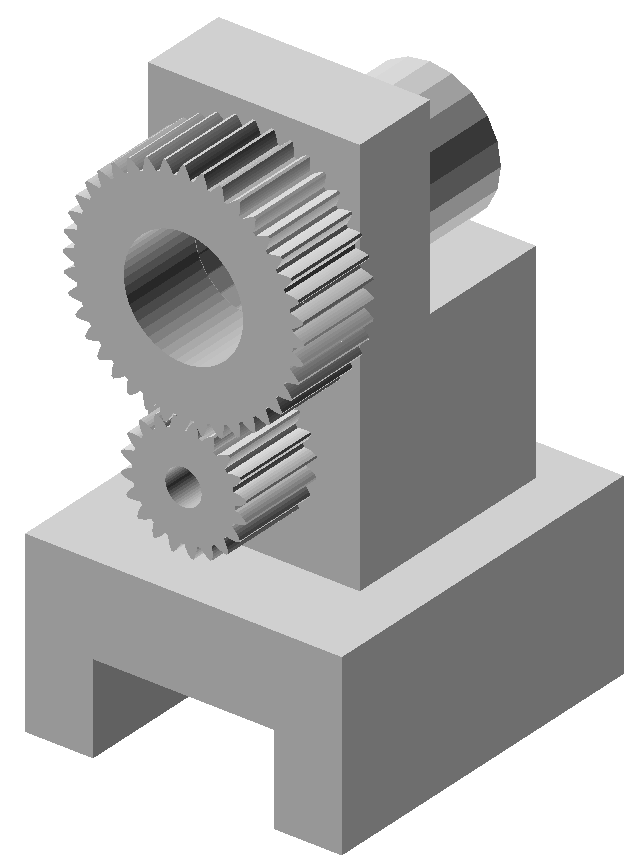
\includegraphics[width=0.8\textwidth]{fig/polarimetro/soporte_all}
                \label{fig:polarimetro/soporte_all}
            \end{figure}
        \end{column}
        \begin{column}{0.5\textwidth}
            \begin{itemize}
                \item Motor NEMA 8 mueve el engranaje inferior paso a paso
                \item Utiliza electrónica creada para el perfilador. Mide en cada paso del motor
                \item Hecho con impresión 3D en plástico
            \end{itemize} 
        \end{column}
    \end{columns}
\end{frame}
